\documentclass[1p]{elsarticle_modified}
%\bibliographystyle{elsarticle-num}

%\usepackage[colorlinks]{hyperref}
%\usepackage{abbrmath_seonhwa} %\Abb, \Ascr, \Acal ,\Abf, \Afrak
\usepackage{amsfonts}
\usepackage{amssymb}
\usepackage{amsmath}
\usepackage{amsthm}
\usepackage{scalefnt}
\usepackage{amsbsy}
\usepackage{kotex}
\usepackage{caption}
\usepackage{subfig}
\usepackage{color}
\usepackage{graphicx}
\usepackage{xcolor} %% white, black, red, green, blue, cyan, magenta, yellow
\usepackage{float}
\usepackage{setspace}
\usepackage{hyperref}

\usepackage{tikz}
\usetikzlibrary{arrows}

\usepackage{multirow}
\usepackage{array} % fixed length table
\usepackage{hhline}

%%%%%%%%%%%%%%%%%%%%%
\makeatletter
\renewcommand*\env@matrix[1][\arraystretch]{%
	\edef\arraystretch{#1}%
	\hskip -\arraycolsep
	\let\@ifnextchar\new@ifnextchar
	\array{*\c@MaxMatrixCols c}}
\makeatother %https://tex.stackexchange.com/questions/14071/how-can-i-increase-the-line-spacing-in-a-matrix
%%%%%%%%%%%%%%%

\usepackage[normalem]{ulem}

\newcommand{\msout}[1]{\ifmmode\text{\sout{\ensuremath{#1}}}\else\sout{#1}\fi}
%SOURCE: \msout is \stkout macro in https://tex.stackexchange.com/questions/20609/strikeout-in-math-mode

\newcommand{\cancel}[1]{
	\ifmmode
	{\color{red}\msout{#1}}
	\else
	{\color{red}\sout{#1}}
	\fi
}

\newcommand{\add}[1]{
	{\color{blue}\uwave{#1}}
}

\newcommand{\replace}[2]{
	\ifmmode
	{\color{red}\msout{#1}}{\color{blue}\uwave{#2}}
	\else
	{\color{red}\sout{#1}}{\color{blue}\uwave{#2}}
	\fi
}

\newcommand{\Sol}{\mathcal{S}} %segment
\newcommand{\D}{D} %diagram
\newcommand{\A}{\mathcal{A}} %arc


%%%%%%%%%%%%%%%%%%%%%%%%%%%%%5 test

\def\sl{\operatorname{\textup{SL}}(2,\Cbb)}
\def\psl{\operatorname{\textup{PSL}}(2,\Cbb)}
\def\quan{\mkern 1mu \triangleright \mkern 1mu}

\theoremstyle{definition}
\newtheorem{thm}{Theorem}[section]
\newtheorem{prop}[thm]{Proposition}
\newtheorem{lem}[thm]{Lemma}
\newtheorem{ques}[thm]{Question}
\newtheorem{cor}[thm]{Corollary}
\newtheorem{defn}[thm]{Definition}
\newtheorem{exam}[thm]{Example}
\newtheorem{rmk}[thm]{Remark}
\newtheorem{alg}[thm]{Algorithm}

\newcommand{\I}{\sqrt{-1}}
\begin{document}

%\begin{frontmatter}
%
%\title{Boundary parabolic representations of knots up to 8 crossings}
%
%%% Group authors per affiliation:
%\author{Yunhi Cho} 
%\address{Department of Mathematics, University of Seoul, Seoul, Korea}
%\ead{yhcho@uos.ac.kr}
%
%
%\author{Seonhwa Kim} %\fnref{s_kim}}
%\address{Center for Geometry and Physics, Institute for Basic Science, Pohang, 37673, Korea}
%\ead{ryeona17@ibs.re.kr}
%
%\author{Hyuk Kim}
%\address{Department of Mathematical Sciences, Seoul National University, Seoul 08826, Korea}
%\ead{hyukkim@snu.ac.kr}
%
%\author{Seokbeom Yoon}
%\address{Department of Mathematical Sciences, Seoul National University, Seoul, 08826,  Korea}
%\ead{sbyoon15@snu.ac.kr}
%
%\begin{abstract}
%We find all boundary parabolic representation of knots up to 8 crossings.
%
%\end{abstract}
%\begin{keyword}
%    \MSC[2010] 57M25 
%\end{keyword}
%
%\end{frontmatter}

%\linenumbers
%\tableofcontents
%
\newcommand\colored[1]{\textcolor{white}{\rule[-0.35ex]{0.8em}{1.4ex}}\kern-0.8em\color{red} #1}%
%\newcommand\colored[1]{\textcolor{white}{ #1}\kern-2.17ex	\textcolor{white}{ #1}\kern-1.81ex	\textcolor{white}{ #1}\kern-2.15ex\color{red}#1	}

{\Large $\underline{12a_{1256}~(K12a_{1256})}$}

\setlength{\tabcolsep}{10pt}
\renewcommand{\arraystretch}{1.6}
\vspace{1cm}\begin{tabular}{m{100pt}>{\centering\arraybackslash}m{274pt}}
\multirow{5}{120pt}{
	\centering
	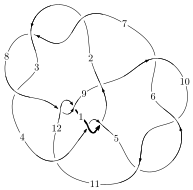
\includegraphics[width=112pt]{../../../GIT/diagram.site/Diagrams/png/2057_12a_1256.png}\\
\ \ \ A knot diagram\footnotemark}&
\allowdisplaybreaks
\textbf{Linearized knot diagam} \\
\cline{2-2}
 &
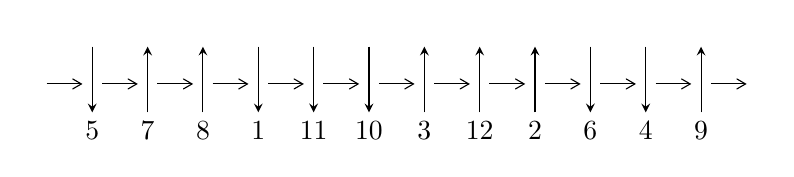
\begin{tikzpicture}[x=20pt, y=17pt]
	% nodes
	\node (C0) at (0, 0) {};
	\node (C1) at (1, 0) {};
	\node (C1U) at (1, +1) {};
	\node (C1D) at (1, -1) {5};

	\node (C2) at (2, 0) {};
	\node (C2U) at (2, +1) {};
	\node (C2D) at (2, -1) {7};

	\node (C3) at (3, 0) {};
	\node (C3U) at (3, +1) {};
	\node (C3D) at (3, -1) {8};

	\node (C4) at (4, 0) {};
	\node (C4U) at (4, +1) {};
	\node (C4D) at (4, -1) {1};

	\node (C5) at (5, 0) {};
	\node (C5U) at (5, +1) {};
	\node (C5D) at (5, -1) {11};

	\node (C6) at (6, 0) {};
	\node (C6U) at (6, +1) {};
	\node (C6D) at (6, -1) {10};

	\node (C7) at (7, 0) {};
	\node (C7U) at (7, +1) {};
	\node (C7D) at (7, -1) {3};

	\node (C8) at (8, 0) {};
	\node (C8U) at (8, +1) {};
	\node (C8D) at (8, -1) {12};

	\node (C9) at (9, 0) {};
	\node (C9U) at (9, +1) {};
	\node (C9D) at (9, -1) {2};

	\node (C10) at (10, 0) {};
	\node (C10U) at (10, +1) {};
	\node (C10D) at (10, -1) {6};

	\node (C11) at (11, 0) {};
	\node (C11U) at (11, +1) {};
	\node (C11D) at (11, -1) {4};

	\node (C12) at (12, 0) {};
	\node (C12U) at (12, +1) {};
	\node (C12D) at (12, -1) {9};
	\node (C13) at (13, 0) {};

	% arrows
	\draw[->,>={angle 60}]
	(C0) edge (C1) (C1) edge (C2) (C2) edge (C3) (C3) edge (C4) (C4) edge (C5) (C5) edge (C6) (C6) edge (C7) (C7) edge (C8) (C8) edge (C9) (C9) edge (C10) (C10) edge (C11) (C11) edge (C12) (C12) edge (C13) ;	\draw[->,>=stealth]
	(C1U) edge (C1D) (C2D) edge (C2U) (C3D) edge (C3U) (C4U) edge (C4D) (C5U) edge (C5D) (C6U) edge (C6D) (C7D) edge (C7U) (C8D) edge (C8U) (C9D) edge (C9U) (C10U) edge (C10D) (C11U) edge (C11D) (C12D) edge (C12U) ;
	\end{tikzpicture} \\
\hhline{~~} \\& 
\textbf{Solving Sequence} \\ \cline{2-2} 
 &
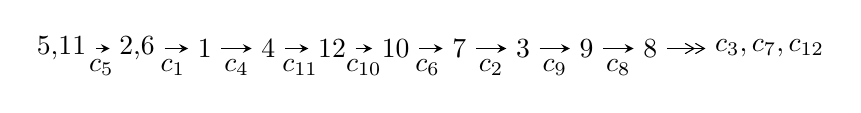
\begin{tikzpicture}[x=23pt, y=7pt]
	% node
	\node (A0) at (-1/8, 0) {5,11};
	\node (A1) at (17/16, 0) {2,6};
	\node (A2) at (17/8, 0) {1};
	\node (A3) at (25/8, 0) {4};
	\node (A4) at (33/8, 0) {12};
	\node (A5) at (41/8, 0) {10};
	\node (A6) at (49/8, 0) {7};
	\node (A7) at (57/8, 0) {3};
	\node (A8) at (65/8, 0) {9};
	\node (A9) at (73/8, 0) {8};
	\node (C1) at (1/2, -1) {$c_{5}$};
	\node (C2) at (13/8, -1) {$c_{1}$};
	\node (C3) at (21/8, -1) {$c_{4}$};
	\node (C4) at (29/8, -1) {$c_{11}$};
	\node (C5) at (37/8, -1) {$c_{10}$};
	\node (C6) at (45/8, -1) {$c_{6}$};
	\node (C7) at (53/8, -1) {$c_{2}$};
	\node (C8) at (61/8, -1) {$c_{9}$};
	\node (C9) at (69/8, -1) {$c_{8}$};
	\node (A10) at (11, 0) {$c_{3},c_{7},c_{12}$};

	% edge
	\draw[->,>=stealth]	
	(A0) edge (A1) (A1) edge (A2) (A2) edge (A3) (A3) edge (A4) (A4) edge (A5) (A5) edge (A6) (A6) edge (A7) (A7) edge (A8) (A8) edge (A9) ;
	\draw[->>,>={angle 60}]	
	(A9) edge (A10);
\end{tikzpicture} \\ 

\end{tabular} \\

\footnotetext{
The image of knot diagram is generated by the software ``\textbf{Draw programme}" developed by Andrew Bartholomew(\url{http://www.layer8.co.uk/maths/draw/index.htm\#Running-draw}), where we modified some parts for our purpose(\url{https://github.com/CATsTAILs/LinksPainter}).
}\phantom \\ \newline 
\centering \textbf{Ideals for irreducible components\footnotemark of $X_{\text{par}}$} 
 
\begin{align*}
I^u_{1}&=\langle 
-5.64042\times10^{124} u^{74}+9.11620\times10^{125} u^{73}+\cdots+2.70123\times10^{127} b+2.73247\times10^{127},\\
\phantom{I^u_{1}}&\phantom{= \langle  }4.87882\times10^{130} u^{74}-9.04411\times10^{130} u^{73}+\cdots+1.18314\times10^{130} a+2.77838\times10^{131},\;u^{75}-2 u^{74}+\cdots+2 u-1\rangle \\
I^u_{2}&=\langle 
b-1,\;3 a^2-4 a u-2 a+2 u-1,\;u^2+u+1\rangle \\
I^u_{3}&=\langle 
b+1,\;3 a-2 u+1,\;u^2- u+1\rangle \\
\\
\end{align*}
\raggedright * 3 irreducible components of $\dim_{\mathbb{C}}=0$, with total 81 representations.\\
\footnotetext{All coefficients of polynomials are rational numbers. But the coefficients are sometimes approximated in decimal forms when there is not enough margin.}
\newpage
\renewcommand{\arraystretch}{1}
\centering \section*{I. $I^u_{1}= \langle -5.64\times10^{124} u^{74}+9.12\times10^{125} u^{73}+\cdots+2.70\times10^{127} b+2.73\times10^{127},\;4.88\times10^{130} u^{74}-9.04\times10^{130} u^{73}+\cdots+1.18\times10^{130} a+2.78\times10^{131},\;u^{75}-2 u^{74}+\cdots+2 u-1 \rangle$}
\flushleft \textbf{(i) Arc colorings}\\
\begin{tabular}{m{7pt} m{180pt} m{7pt} m{180pt} }
\flushright $a_{5}=$&$\begin{pmatrix}1\\0\end{pmatrix}$ \\
\flushright $a_{11}=$&$\begin{pmatrix}0\\u\end{pmatrix}$ \\
\flushright $a_{2}=$&$\begin{pmatrix}-4.12363 u^{74}+7.64417 u^{73}+\cdots-122.730 u-23.4832\\0.00208809 u^{74}-0.0337483 u^{73}+\cdots-0.242348 u-1.01157\end{pmatrix}$ \\
\flushright $a_{6}=$&$\begin{pmatrix}1\\u^2\end{pmatrix}$ \\
\flushright $a_{1}=$&$\begin{pmatrix}-4.12154 u^{74}+7.61042 u^{73}+\cdots-122.972 u-24.4947\\0.00208809 u^{74}-0.0337483 u^{73}+\cdots-0.242348 u-1.01157\end{pmatrix}$ \\
\flushright $a_{4}=$&$\begin{pmatrix}-4.08530 u^{74}+7.78212 u^{73}+\cdots-132.075 u-25.7741\\0.258927 u^{74}-0.465895 u^{73}+\cdots-1.90127 u-0.653622\end{pmatrix}$ \\
\flushright $a_{12}=$&$\begin{pmatrix}-36.6756 u^{74}+67.7990 u^{73}+\cdots-1097.47 u-238.095\\-0.354825 u^{74}+0.662723 u^{73}+\cdots-20.6852 u-4.84533\end{pmatrix}$ \\
\flushright $a_{10}=$&$\begin{pmatrix}u\\u^3+u\end{pmatrix}$ \\
\flushright $a_{7}=$&$\begin{pmatrix}u^2+1\\u^4+2 u^2\end{pmatrix}$ \\
\flushright $a_{3}=$&$\begin{pmatrix}-3.85208 u^{74}+7.11086 u^{73}+\cdots-116.744 u-23.2694\\-0.0278066 u^{74}+0.0198137 u^{73}+\cdots+0.251746 u-0.982130\end{pmatrix}$ \\
\flushright $a_{9}=$&$\begin{pmatrix}-32.4337 u^{74}+60.1196 u^{73}+\cdots-960.246 u-207.404\\-0.475413 u^{74}+0.935445 u^{73}+\cdots-15.5725 u-4.66742\end{pmatrix}$ \\
\flushright $a_{8}=$&$\begin{pmatrix}5.31272 u^{74}-9.69537 u^{73}+\cdots+154.183 u+37.8595\\0.280173 u^{74}-0.556071 u^{73}+\cdots+5.64826 u+0.243813\end{pmatrix}$\\&\end{tabular}
\flushleft \textbf{(ii) Obstruction class $= -1$}\\~\\
\flushleft \textbf{(iii) Cusp Shapes $= -7.72579 u^{74}+14.3690 u^{73}+\cdots-174.823 u-40.1034$}\\~\\
\newpage\renewcommand{\arraystretch}{1}
\flushleft \textbf{(iv) u-Polynomials at the component}\newline \\
\begin{tabular}{m{50pt}|m{274pt}}
Crossings & \hspace{64pt}u-Polynomials at each crossing \\
\hline $$\begin{aligned}c_{1},c_{4}\end{aligned}$$&$\begin{aligned}
&u^{75}+3 u^{74}+\cdots-25 u-63
\end{aligned}$\\
\hline $$\begin{aligned}c_{2},c_{3},c_{7}\end{aligned}$$&$\begin{aligned}
&u^{75}+3 u^{74}+\cdots-180 u+36
\end{aligned}$\\
\hline $$\begin{aligned}c_{5},c_{6},c_{10}\end{aligned}$$&$\begin{aligned}
&u^{75}+2 u^{74}+\cdots+2 u+1
\end{aligned}$\\
\hline $$\begin{aligned}c_{8},c_{12}\end{aligned}$$&$\begin{aligned}
&u^{75}-4 u^{74}+\cdots-12 u-1
\end{aligned}$\\
\hline $$\begin{aligned}c_{9}\end{aligned}$$&$\begin{aligned}
&219(219 u^{75}+2561 u^{74}+\cdots-4.11026\times10^{7} u+9603649)
\end{aligned}$\\
\hline $$\begin{aligned}c_{11}\end{aligned}$$&$\begin{aligned}
&219(219 u^{75}-3206 u^{74}+\cdots+2099664 u-1065445)
\end{aligned}$\\
\hline
\end{tabular}\\~\\
\newpage\renewcommand{\arraystretch}{1}
\flushleft \textbf{(v) Riley Polynomials at the component}\newline \\
\begin{tabular}{m{50pt}|m{274pt}}
Crossings & \hspace{64pt}Riley Polynomials at each crossing \\
\hline $$\begin{aligned}c_{1},c_{4}\end{aligned}$$&$\begin{aligned}
&y^{75}-39 y^{74}+\cdots-12479 y-3969
\end{aligned}$\\
\hline $$\begin{aligned}c_{2},c_{3},c_{7}\end{aligned}$$&$\begin{aligned}
&y^{75}-85 y^{74}+\cdots+21456 y-1296
\end{aligned}$\\
\hline $$\begin{aligned}c_{5},c_{6},c_{10}\end{aligned}$$&$\begin{aligned}
&y^{75}+74 y^{74}+\cdots+48 y-1
\end{aligned}$\\
\hline $$\begin{aligned}c_{8},c_{12}\end{aligned}$$&$\begin{aligned}
&y^{75}-46 y^{74}+\cdots-16 y-1
\end{aligned}$\\
\hline $$\begin{aligned}c_{9}\end{aligned}$$&$\begin{aligned}
&47961(47961 y^{75}-5944207 y^{74}+\cdots+1.71498\times10^{15} y-9.22301\times10^{13})
\end{aligned}$\\
\hline $$\begin{aligned}c_{11}\end{aligned}$$&$\begin{aligned}
&47961\\
&\cdot(47961 y^{75}-1905190 y^{74}+\cdots-29363839817524 y-1135173048025)
\end{aligned}$\\
\hline
\end{tabular}\\~\\
\newpage\flushleft \textbf{(vi) Complex Volumes and Cusp Shapes}
$$\begin{array}{c|c|c}  
\text{Solutions to }I^u_{1}& \I (\text{vol} + \sqrt{-1}CS) & \text{Cusp shape}\\
 \hline 
\begin{aligned}
u &= \phantom{-}0.876275 + 0.562290 I \\
a &= \phantom{-}0.705559 - 0.938222 I \\
b &= \phantom{-}1.235900 + 0.607876 I\end{aligned}
 & \phantom{-}8.0251 - 11.7833 I & \phantom{-0.000000 } 0 \\ \hline\begin{aligned}
u &= \phantom{-}0.876275 - 0.562290 I \\
a &= \phantom{-}0.705559 + 0.938222 I \\
b &= \phantom{-}1.235900 - 0.607876 I\end{aligned}
 & \phantom{-}8.0251 + 11.7833 I & \phantom{-0.000000 } 0 \\ \hline\begin{aligned}
u &= \phantom{-}0.645654 + 0.681122 I \\
a &= -0.141459 + 0.379704 I \\
b &= \phantom{-}0.211314 - 0.993029 I\end{aligned}
 & \phantom{-}11.12440 - 6.04518 I & \phantom{-0.000000 } 0 \\ \hline\begin{aligned}
u &= \phantom{-}0.645654 - 0.681122 I \\
a &= -0.141459 - 0.379704 I \\
b &= \phantom{-}0.211314 + 0.993029 I\end{aligned}
 & \phantom{-}11.12440 + 6.04518 I & \phantom{-0.000000 } 0 \\ \hline\begin{aligned}
u &= \phantom{-}0.869381 + 0.333279 I \\
a &= \phantom{-}0.989488 - 0.311346 I \\
b &= \phantom{-}0.475379 + 0.683609 I\end{aligned}
 & \phantom{-}9.93704 + 1.09383 I & \phantom{-0.000000 } 0 \\ \hline\begin{aligned}
u &= \phantom{-}0.869381 - 0.333279 I \\
a &= \phantom{-}0.989488 + 0.311346 I \\
b &= \phantom{-}0.475379 - 0.683609 I\end{aligned}
 & \phantom{-}9.93704 - 1.09383 I & \phantom{-0.000000 } 0 \\ \hline\begin{aligned}
u &= \phantom{-}0.887065 + 0.671795 I \\
a &= \phantom{-}0.080791 - 0.173949 I \\
b &= \phantom{-}1.043970 - 0.564127 I\end{aligned}
 & \phantom{-}8.26968 + 5.91564 I & \phantom{-0.000000 } 0 \\ \hline\begin{aligned}
u &= \phantom{-}0.887065 - 0.671795 I \\
a &= \phantom{-}0.080791 + 0.173949 I \\
b &= \phantom{-}1.043970 + 0.564127 I\end{aligned}
 & \phantom{-}8.26968 - 5.91564 I & \phantom{-0.000000 } 0 \\ \hline\begin{aligned}
u &= \phantom{-}0.617922 + 0.932156 I \\
a &= -0.091814 + 0.364728 I \\
b &= -0.900452 + 0.105348 I\end{aligned}
 & -1.38488 - 1.76088 I & \phantom{-0.000000 } 0 \\ \hline\begin{aligned}
u &= \phantom{-}0.617922 - 0.932156 I \\
a &= -0.091814 - 0.364728 I \\
b &= -0.900452 - 0.105348 I\end{aligned}
 & -1.38488 + 1.76088 I & \phantom{-0.000000 } 0\\
 \hline 
 \end{array}$$\newpage$$\begin{array}{c|c|c}  
\text{Solutions to }I^u_{1}& \I (\text{vol} + \sqrt{-1}CS) & \text{Cusp shape}\\
 \hline 
\begin{aligned}
u &= -0.630870 + 0.610023 I \\
a &= \phantom{-}0.209312 - 0.433808 I \\
b &= -1.020630 - 0.440018 I\end{aligned}
 & \phantom{-}1.00908 - 3.90722 I & \phantom{-0.000000 } 0 \\ \hline\begin{aligned}
u &= -0.630870 - 0.610023 I \\
a &= \phantom{-}0.209312 + 0.433808 I \\
b &= -1.020630 + 0.440018 I\end{aligned}
 & \phantom{-}1.00908 + 3.90722 I & \phantom{-0.000000 } 0 \\ \hline\begin{aligned}
u &= \phantom{-}0.781439 + 0.396315 I \\
a &= -0.681940 + 0.719996 I \\
b &= -1.063160 - 0.318737 I\end{aligned}
 & -2.82400 - 3.24021 I & \phantom{-0.000000 } 0 \\ \hline\begin{aligned}
u &= \phantom{-}0.781439 - 0.396315 I \\
a &= -0.681940 - 0.719996 I \\
b &= -1.063160 + 0.318737 I\end{aligned}
 & -2.82400 + 3.24021 I & \phantom{-0.000000 } 0 \\ \hline\begin{aligned}
u &= -0.200166 + 1.112240 I \\
a &= -0.555735 + 0.472886 I \\
b &= \phantom{-}1.303290 - 0.017947 I\end{aligned}
 & \phantom{-}0.00341 + 2.25841 I & \phantom{-0.000000 } 0 \\ \hline\begin{aligned}
u &= -0.200166 - 1.112240 I \\
a &= -0.555735 - 0.472886 I \\
b &= \phantom{-}1.303290 + 0.017947 I\end{aligned}
 & \phantom{-}0.00341 - 2.25841 I & \phantom{-0.000000 } 0 \\ \hline\begin{aligned}
u &= -1.008550 + 0.522926 I \\
a &= \phantom{-}0.622760 + 0.595151 I \\
b &= \phantom{-}0.988198 - 0.455399 I\end{aligned}
 & \phantom{-}3.78624 + 4.97496 I & \phantom{-0.000000 } 0 \\ \hline\begin{aligned}
u &= -1.008550 - 0.522926 I \\
a &= \phantom{-}0.622760 - 0.595151 I \\
b &= \phantom{-}0.988198 + 0.455399 I\end{aligned}
 & \phantom{-}3.78624 - 4.97496 I & \phantom{-0.000000 } 0 \\ \hline\begin{aligned}
u &= -0.715363 + 0.463662 I \\
a &= -0.662169 - 0.968737 I \\
b &= -1.207050 + 0.599270 I\end{aligned}
 & \phantom{-}0.55943 + 8.51493 I & \phantom{-0.000000 } 0 \\ \hline\begin{aligned}
u &= -0.715363 - 0.463662 I \\
a &= -0.662169 + 0.968737 I \\
b &= -1.207050 - 0.599270 I\end{aligned}
 & \phantom{-}0.55943 - 8.51493 I & \phantom{-0.000000 } 0\\
 \hline 
 \end{array}$$\newpage$$\begin{array}{c|c|c}  
\text{Solutions to }I^u_{1}& \I (\text{vol} + \sqrt{-1}CS) & \text{Cusp shape}\\
 \hline 
\begin{aligned}
u &= -0.295177 + 0.790335 I \\
a &= \phantom{-}1.085820 - 0.610170 I \\
b &= -0.174335 + 0.231695 I\end{aligned}
 & \phantom{-}5.11741 + 2.09681 I & \phantom{-0.000000 } 0 \\ \hline\begin{aligned}
u &= -0.295177 - 0.790335 I \\
a &= \phantom{-}1.085820 + 0.610170 I \\
b &= -0.174335 - 0.231695 I\end{aligned}
 & \phantom{-}5.11741 - 2.09681 I & \phantom{-0.000000 } 0 \\ \hline\begin{aligned}
u &= -0.820615 + 0.920549 I \\
a &= \phantom{-}0.221481 + 0.060826 I \\
b &= \phantom{-}0.669207 + 0.351108 I\end{aligned}
 & \phantom{-}4.93623 + 1.38385 I & \phantom{-0.000000 } 0 \\ \hline\begin{aligned}
u &= -0.820615 - 0.920549 I \\
a &= \phantom{-}0.221481 - 0.060826 I \\
b &= \phantom{-}0.669207 - 0.351108 I\end{aligned}
 & \phantom{-}4.93623 - 1.38385 I & \phantom{-0.000000 } 0 \\ \hline\begin{aligned}
u &= \phantom{-}0.476482 + 0.349271 I \\
a &= \phantom{-}0.536263 - 0.913748 I \\
b &= \phantom{-}1.179300 + 0.646970 I\end{aligned}
 & -0.37836 - 3.63250 I & \phantom{-}0.18820 + 7.11754 I \\ \hline\begin{aligned}
u &= \phantom{-}0.476482 - 0.349271 I \\
a &= \phantom{-}0.536263 + 0.913748 I \\
b &= \phantom{-}1.179300 - 0.646970 I\end{aligned}
 & -0.37836 + 3.63250 I & \phantom{-}0.18820 - 7.11754 I \\ \hline\begin{aligned}
u &= -0.12416 + 1.40957 I \\
a &= -0.49322 + 1.49192 I \\
b &= \phantom{-}1.156720 - 0.514868 I\end{aligned}
 & \phantom{-}2.45398 + 2.51607 I & \phantom{-0.000000 } 0 \\ \hline\begin{aligned}
u &= -0.12416 - 1.40957 I \\
a &= -0.49322 - 1.49192 I \\
b &= \phantom{-}1.156720 + 0.514868 I\end{aligned}
 & \phantom{-}2.45398 - 2.51607 I & \phantom{-0.000000 } 0 \\ \hline\begin{aligned}
u &= \phantom{-}0.06595 + 1.41816 I \\
a &= -1.06518 - 1.97261 I \\
b &= \phantom{-}0.726970 + 0.104746 I\end{aligned}
 & \phantom{-}5.61190 - 0.24157 I & \phantom{-0.000000 } 0 \\ \hline\begin{aligned}
u &= \phantom{-}0.06595 - 1.41816 I \\
a &= -1.06518 + 1.97261 I \\
b &= \phantom{-}0.726970 - 0.104746 I\end{aligned}
 & \phantom{-}5.61190 + 0.24157 I & \phantom{-0.000000 } 0\\
 \hline 
 \end{array}$$\newpage$$\begin{array}{c|c|c}  
\text{Solutions to }I^u_{1}& \I (\text{vol} + \sqrt{-1}CS) & \text{Cusp shape}\\
 \hline 
\begin{aligned}
u &= -0.21401 + 1.41679 I \\
a &= -0.32012 - 1.44823 I \\
b &= -0.818643 + 0.496806 I\end{aligned}
 & \phantom{-}7.77805 + 2.57329 I & \phantom{-0.000000 } 0 \\ \hline\begin{aligned}
u &= -0.21401 - 1.41679 I \\
a &= -0.32012 + 1.44823 I \\
b &= -0.818643 - 0.496806 I\end{aligned}
 & \phantom{-}7.77805 - 2.57329 I & \phantom{-0.000000 } 0 \\ \hline\begin{aligned}
u &= -0.318983 + 0.457075 I \\
a &= \phantom{-}0.073646 + 0.417549 I \\
b &= -0.203568 - 1.059760 I\end{aligned}
 & \phantom{-}3.56627 + 2.77566 I & \phantom{-}7.45932 - 8.59352 I \\ \hline\begin{aligned}
u &= -0.318983 - 0.457075 I \\
a &= \phantom{-}0.073646 - 0.417549 I \\
b &= -0.203568 + 1.059760 I\end{aligned}
 & \phantom{-}3.56627 - 2.77566 I & \phantom{-}7.45932 + 8.59352 I \\ \hline\begin{aligned}
u &= -0.02663 + 1.44552 I \\
a &= \phantom{-}0.33553 + 1.40138 I \\
b &= -1.237260 - 0.349849 I\end{aligned}
 & \phantom{-}8.55739 + 0.60577 I & \phantom{-0.000000 } 0 \\ \hline\begin{aligned}
u &= -0.02663 - 1.44552 I \\
a &= \phantom{-}0.33553 - 1.40138 I \\
b &= -1.237260 + 0.349849 I\end{aligned}
 & \phantom{-}8.55739 - 0.60577 I & \phantom{-0.000000 } 0 \\ \hline\begin{aligned}
u &= -0.509960 + 0.186306 I \\
a &= -1.86666 - 0.33094 I \\
b &= -0.427581 + 0.394554 I\end{aligned}
 & \phantom{-}2.65696 - 0.21953 I & \phantom{-}3.66100 - 2.90140 I \\ \hline\begin{aligned}
u &= -0.509960 - 0.186306 I \\
a &= -1.86666 + 0.33094 I \\
b &= -0.427581 - 0.394554 I\end{aligned}
 & \phantom{-}2.65696 + 0.21953 I & \phantom{-}3.66100 + 2.90140 I \\ \hline\begin{aligned}
u &= \phantom{-}0.13294 + 1.45442 I \\
a &= -0.70369 - 1.75188 I \\
b &= \phantom{-}1.30725 + 1.04690 I\end{aligned}
 & \phantom{-}5.48724 - 5.77129 I & \phantom{-0.000000 } 0 \\ \hline\begin{aligned}
u &= \phantom{-}0.13294 - 1.45442 I \\
a &= -0.70369 + 1.75188 I \\
b &= \phantom{-}1.30725 - 1.04690 I\end{aligned}
 & \phantom{-}5.48724 + 5.77129 I & \phantom{-0.000000 } 0\\
 \hline 
 \end{array}$$\newpage$$\begin{array}{c|c|c}  
\text{Solutions to }I^u_{1}& \I (\text{vol} + \sqrt{-1}CS) & \text{Cusp shape}\\
 \hline 
\begin{aligned}
u &= -0.501413 + 0.173375 I \\
a &= \phantom{-}1.18080 + 0.88385 I \\
b &= \phantom{-}1.178950 - 0.178137 I\end{aligned}
 & -2.66084 + 0.41205 I & -3.72410 + 2.82659 I \\ \hline\begin{aligned}
u &= -0.501413 - 0.173375 I \\
a &= \phantom{-}1.18080 - 0.88385 I \\
b &= \phantom{-}1.178950 + 0.178137 I\end{aligned}
 & -2.66084 - 0.41205 I & -3.72410 - 2.82659 I \\ \hline\begin{aligned}
u &= \phantom{-}0.07244 + 1.46773 I \\
a &= \phantom{-}0.129197 - 1.212420 I \\
b &= -0.164854 + 0.790449 I\end{aligned}
 & \phantom{-}6.08949 - 1.95344 I & \phantom{-0.000000 } 0 \\ \hline\begin{aligned}
u &= \phantom{-}0.07244 - 1.46773 I \\
a &= \phantom{-}0.129197 + 1.212420 I \\
b &= -0.164854 - 0.790449 I\end{aligned}
 & \phantom{-}6.08949 + 1.95344 I & \phantom{-0.000000 } 0 \\ \hline\begin{aligned}
u &= -0.07739 + 1.48364 I \\
a &= \phantom{-}0.47777 + 1.88720 I \\
b &= -0.38939 - 1.65589 I\end{aligned}
 & \phantom{-}9.90796 + 4.12833 I & \phantom{-0.000000 } 0 \\ \hline\begin{aligned}
u &= -0.07739 - 1.48364 I \\
a &= \phantom{-}0.47777 - 1.88720 I \\
b &= -0.38939 + 1.65589 I\end{aligned}
 & \phantom{-}9.90796 - 4.12833 I & \phantom{-0.000000 } 0 \\ \hline\begin{aligned}
u &= \phantom{-}0.02616 + 1.48660 I \\
a &= \phantom{-}1.37108 - 0.93149 I \\
b &= -2.00675 + 0.80274 I\end{aligned}
 & \phantom{-}12.23390 - 1.45071 I & \phantom{-0.000000 } 0 \\ \hline\begin{aligned}
u &= \phantom{-}0.02616 - 1.48660 I \\
a &= \phantom{-}1.37108 + 0.93149 I \\
b &= -2.00675 - 0.80274 I\end{aligned}
 & \phantom{-}12.23390 + 1.45071 I & \phantom{-0.000000 } 0 \\ \hline\begin{aligned}
u &= \phantom{-}0.25514 + 1.48012 I \\
a &= \phantom{-}0.25389 + 1.43353 I \\
b &= -1.160740 - 0.553557 I\end{aligned}
 & \phantom{-}3.26790 - 6.92996 I & \phantom{-0.000000 } 0 \\ \hline\begin{aligned}
u &= \phantom{-}0.25514 - 1.48012 I \\
a &= \phantom{-}0.25389 - 1.43353 I \\
b &= -1.160740 + 0.553557 I\end{aligned}
 & \phantom{-}3.26790 + 6.92996 I & \phantom{-0.000000 } 0\\
 \hline 
 \end{array}$$\newpage$$\begin{array}{c|c|c}  
\text{Solutions to }I^u_{1}& \I (\text{vol} + \sqrt{-1}CS) & \text{Cusp shape}\\
 \hline 
\begin{aligned}
u &= -0.11892 + 1.50576 I \\
a &= \phantom{-}0.824177 + 0.454392 I \\
b &= -0.704332 - 0.473961 I\end{aligned}
 & \phantom{-}8.08900 - 1.43331 I & \phantom{-0.000000 } 0 \\ \hline\begin{aligned}
u &= -0.11892 - 1.50576 I \\
a &= \phantom{-}0.824177 - 0.454392 I \\
b &= -0.704332 + 0.473961 I\end{aligned}
 & \phantom{-}8.08900 + 1.43331 I & \phantom{-0.000000 } 0 \\ \hline\begin{aligned}
u &= -0.24148 + 1.50171 I \\
a &= \phantom{-}0.38547 - 1.69930 I \\
b &= -1.30554 + 0.78742 I\end{aligned}
 & \phantom{-}6.96349 + 11.98440 I & \phantom{-0.000000 } 0 \\ \hline\begin{aligned}
u &= -0.24148 - 1.50171 I \\
a &= \phantom{-}0.38547 + 1.69930 I \\
b &= -1.30554 - 0.78742 I\end{aligned}
 & \phantom{-}6.96349 - 11.98440 I & \phantom{-0.000000 } 0 \\ \hline\begin{aligned}
u &= \phantom{-}0.290488 + 0.380055 I \\
a &= -1.87771 - 2.07115 I \\
b &= \phantom{-}0.958564 - 0.242001 I\end{aligned}
 & \phantom{-}0.033322 + 0.939980 I & -0.28548 + 8.35060 I \\ \hline\begin{aligned}
u &= \phantom{-}0.290488 - 0.380055 I \\
a &= -1.87771 + 2.07115 I \\
b &= \phantom{-}0.958564 + 0.242001 I\end{aligned}
 & \phantom{-}0.033322 - 0.939980 I & -0.28548 - 8.35060 I \\ \hline\begin{aligned}
u &= \phantom{-}0.246631 + 0.362441 I \\
a &= -0.412210 - 0.560123 I \\
b &= \phantom{-}0.095378 + 0.306837 I\end{aligned}
 & \phantom{-}0.022305 - 0.818920 I & \phantom{-}0.60380 + 8.33349 I \\ \hline\begin{aligned}
u &= \phantom{-}0.246631 - 0.362441 I \\
a &= -0.412210 + 0.560123 I \\
b &= \phantom{-}0.095378 - 0.306837 I\end{aligned}
 & \phantom{-}0.022305 + 0.818920 I & \phantom{-}0.60380 - 8.33349 I \\ \hline\begin{aligned}
u &= \phantom{-}0.38353 + 1.51514 I \\
a &= \phantom{-}0.343106 - 1.142940 I \\
b &= \phantom{-}0.865449 + 0.692400 I\end{aligned}
 & \phantom{-}15.8330 - 3.6081 I & \phantom{-0.000000 } 0 \\ \hline\begin{aligned}
u &= \phantom{-}0.38353 - 1.51514 I \\
a &= \phantom{-}0.343106 + 1.142940 I \\
b &= \phantom{-}0.865449 - 0.692400 I\end{aligned}
 & \phantom{-}15.8330 + 3.6081 I & \phantom{-0.000000 } 0\\
 \hline 
 \end{array}$$\newpage$$\begin{array}{c|c|c}  
\text{Solutions to }I^u_{1}& \I (\text{vol} + \sqrt{-1}CS) & \text{Cusp shape}\\
 \hline 
\begin{aligned}
u &= \phantom{-}0.129313 + 0.412192 I \\
a &= -0.761012 - 0.474573 I \\
b &= -1.48075 + 0.50912 I\end{aligned}
 & \phantom{-}5.94006 - 0.95777 I & \phantom{-}13.8115 + 6.3144 I \\ \hline\begin{aligned}
u &= \phantom{-}0.129313 - 0.412192 I \\
a &= -0.761012 + 0.474573 I \\
b &= -1.48075 - 0.50912 I\end{aligned}
 & \phantom{-}5.94006 + 0.95777 I & \phantom{-}13.8115 - 6.3144 I \\ \hline\begin{aligned}
u &= \phantom{-}0.19790 + 1.57054 I \\
a &= -0.45227 + 1.42247 I \\
b &= \phantom{-}0.201938 - 1.324450 I\end{aligned}
 & \phantom{-}18.5743 - 9.1429 I & \phantom{-0.000000 } 0 \\ \hline\begin{aligned}
u &= \phantom{-}0.19790 - 1.57054 I \\
a &= -0.45227 - 1.42247 I \\
b &= \phantom{-}0.201938 + 1.324450 I\end{aligned}
 & \phantom{-}18.5743 + 9.1429 I & \phantom{-0.000000 } 0 \\ \hline\begin{aligned}
u &= \phantom{-}0.30448 + 1.56248 I \\
a &= -0.18734 - 1.61409 I \\
b &= \phantom{-}1.35622 + 0.69432 I\end{aligned}
 & \phantom{-}14.9505 - 16.1112 I & \phantom{-0.000000 } 0 \\ \hline\begin{aligned}
u &= \phantom{-}0.30448 - 1.56248 I \\
a &= -0.18734 + 1.61409 I \\
b &= \phantom{-}1.35622 - 0.69432 I\end{aligned}
 & \phantom{-}14.9505 + 16.1112 I & \phantom{-0.000000 } 0 \\ \hline\begin{aligned}
u &= -0.17402 + 1.59685 I \\
a &= -0.163007 - 1.070100 I \\
b &= \phantom{-}0.276738 + 0.882519 I\end{aligned}
 & \phantom{-}13.38520 + 4.43309 I & \phantom{-0.000000 } 0 \\ \hline\begin{aligned}
u &= -0.17402 - 1.59685 I \\
a &= -0.163007 + 1.070100 I \\
b &= \phantom{-}0.276738 - 0.882519 I\end{aligned}
 & \phantom{-}13.38520 - 4.43309 I & \phantom{-0.000000 } 0 \\ \hline\begin{aligned}
u &= -0.33867 + 1.58027 I \\
a &= -0.107663 + 1.311530 I \\
b &= \phantom{-}1.184290 - 0.597745 I\end{aligned}
 & \phantom{-}10.6747 + 9.8638 I & \phantom{-0.000000 } 0 \\ \hline\begin{aligned}
u &= -0.33867 - 1.58027 I \\
a &= -0.107663 - 1.311530 I \\
b &= \phantom{-}1.184290 + 0.597745 I\end{aligned}
 & \phantom{-}10.6747 - 9.8638 I & \phantom{-0.000000 } 0\\
 \hline 
 \end{array}$$\newpage$$\begin{array}{c|c|c}  
\text{Solutions to }I^u_{1}& \I (\text{vol} + \sqrt{-1}CS) & \text{Cusp shape}\\
 \hline 
\begin{aligned}
u &= \phantom{-}0.22442 + 1.64310 I \\
a &= -0.436152 + 0.582597 I \\
b &= \phantom{-}0.746431 - 0.718512 I\end{aligned}
 & \phantom{-}16.1817 + 1.7243 I & \phantom{-0.000000 } 0 \\ \hline\begin{aligned}
u &= \phantom{-}0.22442 - 1.64310 I \\
a &= -0.436152 - 0.582597 I \\
b &= \phantom{-}0.746431 + 0.718512 I\end{aligned}
 & \phantom{-}16.1817 - 1.7243 I & \phantom{-0.000000 } 0 \\ \hline\begin{aligned}
u &= -0.243105 + 0.095142 I \\
a &= \phantom{-}2.59239 + 2.02032 I \\
b &= -0.861746 - 0.111814 I\end{aligned}
 & \phantom{-}3.19638 + 0.01813 I & \phantom{-}0.93086 + 1.13023 I \\ \hline\begin{aligned}
u &= -0.243105 - 0.095142 I \\
a &= \phantom{-}2.59239 - 2.02032 I \\
b &= -0.861746 + 0.111814 I\end{aligned}
 & \phantom{-}3.19638 - 0.01813 I & \phantom{-}0.93086 - 1.13023 I \\ \hline\begin{aligned}
u &= \phantom{-}0.151778\phantom{ +0.000000I} \\
a &= -54.3761\phantom{ +0.000000I} \\
b &= -1.06936\phantom{ +0.000000I}\end{aligned}
 & \phantom{-}4.98695\phantom{ +0.000000I} & -85.6430\phantom{ +0.000000I}\\
 \hline 
 \end{array}$$\newpage\newpage\renewcommand{\arraystretch}{1}
\centering \section*{II. $I^u_{2}= \langle b-1,\;3 a^2-4 a u-2 a+2 u-1,\;u^2+u+1 \rangle$}
\flushleft \textbf{(i) Arc colorings}\\
\begin{tabular}{m{7pt} m{180pt} m{7pt} m{180pt} }
\flushright $a_{5}=$&$\begin{pmatrix}1\\0\end{pmatrix}$ \\
\flushright $a_{11}=$&$\begin{pmatrix}0\\u\end{pmatrix}$ \\
\flushright $a_{2}=$&$\begin{pmatrix}a\\1\end{pmatrix}$ \\
\flushright $a_{6}=$&$\begin{pmatrix}1\\- u-1\end{pmatrix}$ \\
\flushright $a_{1}=$&$\begin{pmatrix}a+1\\1\end{pmatrix}$ \\
\flushright $a_{4}=$&$\begin{pmatrix}- a\\-1\end{pmatrix}$ \\
\flushright $a_{12}=$&$\begin{pmatrix}\frac{2}{3} a u+\frac{4}{3} a- u-\frac{2}{3}\\- a u+u\end{pmatrix}$ \\
\flushright $a_{10}=$&$\begin{pmatrix}u\\u+1\end{pmatrix}$ \\
\flushright $a_{7}=$&$\begin{pmatrix}- u\\- u-2\end{pmatrix}$ \\
\flushright $a_{3}=$&$\begin{pmatrix}- a u+2 a- u-1\\-3 a u-3 a+u\end{pmatrix}$ \\
\flushright $a_{9}=$&$\begin{pmatrix}\frac{1}{3} a u+\frac{2}{3} a+\frac{2}{3} u-1\\- a u- a+2 u+1\end{pmatrix}$ \\
\flushright $a_{8}=$&$\begin{pmatrix}- a u+\frac{4}{3} u-\frac{4}{3}\\- a u-2 a+2 u+2\end{pmatrix}$\\&\end{tabular}
\flushleft \textbf{(ii) Obstruction class $= 1$}\\~\\
\flushleft \textbf{(iii) Cusp Shapes $= -4 u$}\\~\\
\newpage\renewcommand{\arraystretch}{1}
\flushleft \textbf{(iv) u-Polynomials at the component}\newline \\
\begin{tabular}{m{50pt}|m{274pt}}
Crossings & \hspace{64pt}u-Polynomials at each crossing \\
\hline $$\begin{aligned}c_{1}\end{aligned}$$&$\begin{aligned}
&(u+1)^4
\end{aligned}$\\
\hline $$\begin{aligned}c_{2},c_{3},c_{7}\end{aligned}$$&$\begin{aligned}
&(u^2-2)^2
\end{aligned}$\\
\hline $$\begin{aligned}c_{4}\end{aligned}$$&$\begin{aligned}
&(u-1)^4
\end{aligned}$\\
\hline $$\begin{aligned}c_{5},c_{6},c_{8}\end{aligned}$$&$\begin{aligned}
&(u^2+u+1)^2
\end{aligned}$\\
\hline $$\begin{aligned}c_{9}\end{aligned}$$&$\begin{aligned}
&9(9 u^4+12 u+7)
\end{aligned}$\\
\hline $$\begin{aligned}c_{10},c_{12}\end{aligned}$$&$\begin{aligned}
&(u^2- u+1)^2
\end{aligned}$\\
\hline $$\begin{aligned}c_{11}\end{aligned}$$&$\begin{aligned}
&9(9 u^4+18 u^3+27 u^2+18 u+7)
\end{aligned}$\\
\hline
\end{tabular}\\~\\
\newpage\renewcommand{\arraystretch}{1}
\flushleft \textbf{(v) Riley Polynomials at the component}\newline \\
\begin{tabular}{m{50pt}|m{274pt}}
Crossings & \hspace{64pt}Riley Polynomials at each crossing \\
\hline $$\begin{aligned}c_{1},c_{4}\end{aligned}$$&$\begin{aligned}
&(y-1)^4
\end{aligned}$\\
\hline $$\begin{aligned}c_{2},c_{3},c_{7}\end{aligned}$$&$\begin{aligned}
&(y-2)^4
\end{aligned}$\\
\hline $$\begin{aligned}c_{5},c_{6},c_{8}\\c_{10},c_{12}\end{aligned}$$&$\begin{aligned}
&(y^2+y+1)^2
\end{aligned}$\\
\hline $$\begin{aligned}c_{9}\end{aligned}$$&$\begin{aligned}
&81(81 y^4+126 y^2-144 y+49)
\end{aligned}$\\
\hline $$\begin{aligned}c_{11}\end{aligned}$$&$\begin{aligned}
&81(81 y^4+162 y^3+207 y^2+54 y+49)
\end{aligned}$\\
\hline
\end{tabular}\\~\\
\newpage\flushleft \textbf{(vi) Complex Volumes and Cusp Shapes}
$$\begin{array}{c|c|c}  
\text{Solutions to }I^u_{2}& \I (\text{vol} + \sqrt{-1}CS) & \text{Cusp shape}\\
 \hline 
\begin{aligned}
u &= -0.500000 + 0.866025 I \\
a &= -0.707107 + 0.985599 I \\
b &= \phantom{-}1.00000\phantom{ +0.000000I}\end{aligned}
 & \phantom{-}3.28987 + 2.02988 I & \phantom{-}2.00000 - 3.46410 I \\ \hline\begin{aligned}
u &= -0.500000 + 0.866025 I \\
a &= \phantom{-}0.707107 + 0.169102 I \\
b &= \phantom{-}1.00000\phantom{ +0.000000I}\end{aligned}
 & \phantom{-}3.28987 + 2.02988 I & \phantom{-}2.00000 - 3.46410 I \\ \hline\begin{aligned}
u &= -0.500000 - 0.866025 I \\
a &= -0.707107 - 0.985599 I \\
b &= \phantom{-}1.00000\phantom{ +0.000000I}\end{aligned}
 & \phantom{-}3.28987 - 2.02988 I & \phantom{-}2.00000 + 3.46410 I \\ \hline\begin{aligned}
u &= -0.500000 - 0.866025 I \\
a &= \phantom{-}0.707107 - 0.169102 I \\
b &= \phantom{-}1.00000\phantom{ +0.000000I}\end{aligned}
 & \phantom{-}3.28987 - 2.02988 I & \phantom{-}2.00000 + 3.46410 I\\
 \hline 
 \end{array}$$\newpage\newpage\renewcommand{\arraystretch}{1}
\centering \section*{III. $I^u_{3}= \langle b+1,\;3 a-2 u+1,\;u^2- u+1 \rangle$}
\flushleft \textbf{(i) Arc colorings}\\
\begin{tabular}{m{7pt} m{180pt} m{7pt} m{180pt} }
\flushright $a_{5}=$&$\begin{pmatrix}1\\0\end{pmatrix}$ \\
\flushright $a_{11}=$&$\begin{pmatrix}0\\u\end{pmatrix}$ \\
\flushright $a_{2}=$&$\begin{pmatrix}\frac{2}{3} u-\frac{1}{3}\\-1\end{pmatrix}$ \\
\flushright $a_{6}=$&$\begin{pmatrix}1\\u-1\end{pmatrix}$ \\
\flushright $a_{1}=$&$\begin{pmatrix}\frac{2}{3} u-\frac{4}{3}\\-1\end{pmatrix}$ \\
\flushright $a_{4}=$&$\begin{pmatrix}\frac{2}{3} u-\frac{1}{3}\\-1\end{pmatrix}$ \\
\flushright $a_{12}=$&$\begin{pmatrix}\frac{1}{3} u\\\frac{4}{3} u-\frac{2}{3}\end{pmatrix}$ \\
\flushright $a_{10}=$&$\begin{pmatrix}u\\u-1\end{pmatrix}$ \\
\flushright $a_{7}=$&$\begin{pmatrix}u\\u-2\end{pmatrix}$ \\
\flushright $a_{3}=$&$\begin{pmatrix}\frac{2}{3} u-\frac{1}{3}\\-1\end{pmatrix}$ \\
\flushright $a_{9}=$&$\begin{pmatrix}u+\frac{1}{3}\\\frac{5}{3} u-\frac{4}{3}\end{pmatrix}$ \\
\flushright $a_{8}=$&$\begin{pmatrix}u\\u-2\end{pmatrix}$\\&\end{tabular}
\flushleft \textbf{(ii) Obstruction class $= 1$}\\~\\
\flushleft \textbf{(iii) Cusp Shapes $= \frac{28}{3} u-10$}\\~\\
\newpage\renewcommand{\arraystretch}{1}
\flushleft \textbf{(iv) u-Polynomials at the component}\newline \\
\begin{tabular}{m{50pt}|m{274pt}}
Crossings & \hspace{64pt}u-Polynomials at each crossing \\
\hline $$\begin{aligned}c_{1}\end{aligned}$$&$\begin{aligned}
&(u-1)^2
\end{aligned}$\\
\hline $$\begin{aligned}c_{2},c_{3},c_{7}\end{aligned}$$&$\begin{aligned}
&u^2
\end{aligned}$\\
\hline $$\begin{aligned}c_{4}\end{aligned}$$&$\begin{aligned}
&(u+1)^2
\end{aligned}$\\
\hline $$\begin{aligned}c_{5},c_{6},c_{12}\end{aligned}$$&$\begin{aligned}
&u^2- u+1
\end{aligned}$\\
\hline $$\begin{aligned}c_{8},c_{10}\end{aligned}$$&$\begin{aligned}
&u^2+u+1
\end{aligned}$\\
\hline $$\begin{aligned}c_{9}\end{aligned}$$&$\begin{aligned}
&3(3 u^2+1)
\end{aligned}$\\
\hline $$\begin{aligned}c_{11}\end{aligned}$$&$\begin{aligned}
&3(3 u^2-3 u+1)
\end{aligned}$\\
\hline
\end{tabular}\\~\\
\newpage\renewcommand{\arraystretch}{1}
\flushleft \textbf{(v) Riley Polynomials at the component}\newline \\
\begin{tabular}{m{50pt}|m{274pt}}
Crossings & \hspace{64pt}Riley Polynomials at each crossing \\
\hline $$\begin{aligned}c_{1},c_{4}\end{aligned}$$&$\begin{aligned}
&(y-1)^2
\end{aligned}$\\
\hline $$\begin{aligned}c_{2},c_{3},c_{7}\end{aligned}$$&$\begin{aligned}
&y^2
\end{aligned}$\\
\hline $$\begin{aligned}c_{5},c_{6},c_{8}\\c_{10},c_{12}\end{aligned}$$&$\begin{aligned}
&y^2+y+1
\end{aligned}$\\
\hline $$\begin{aligned}c_{9}\end{aligned}$$&$\begin{aligned}
&9(3 y+1)^2
\end{aligned}$\\
\hline $$\begin{aligned}c_{11}\end{aligned}$$&$\begin{aligned}
&9(9 y^2-3 y+1)
\end{aligned}$\\
\hline
\end{tabular}\\~\\
\newpage\flushleft \textbf{(vi) Complex Volumes and Cusp Shapes}
$$\begin{array}{c|c|c}  
\text{Solutions to }I^u_{3}& \I (\text{vol} + \sqrt{-1}CS) & \text{Cusp shape}\\
 \hline 
\begin{aligned}
u &= \phantom{-}0.500000 + 0.866025 I \\
a &= \phantom{-0.000000 -}0.577350 I \\
b &= -1.00000\phantom{ +0.000000I}\end{aligned}
 & -1.64493 - 2.02988 I & -5.33333 + 8.08290 I \\ \hline\begin{aligned}
u &= \phantom{-}0.500000 - 0.866025 I \\
a &= \phantom{-0.000000 } -0.577350 I \\
b &= -1.00000\phantom{ +0.000000I}\end{aligned}
 & -1.64493 + 2.02988 I & -5.33333 - 8.08290 I\\
 \hline 
 \end{array}$$\newpage
\newpage\renewcommand{\arraystretch}{1}
\centering \section*{ IV. u-Polynomials}
\begin{tabular}{m{50pt}|m{274pt}}
Crossings & \hspace{64pt}u-Polynomials at each crossing \\
\hline $$\begin{aligned}c_{1}\end{aligned}$$&$\begin{aligned}
&((u-1)^2)(u+1)^4(u^{75}+3 u^{74}+\cdots-25 u-63)
\end{aligned}$\\
\hline $$\begin{aligned}c_{2},c_{3},c_{7}\end{aligned}$$&$\begin{aligned}
&u^2(u^2-2)^2(u^{75}+3 u^{74}+\cdots-180 u+36)
\end{aligned}$\\
\hline $$\begin{aligned}c_{4}\end{aligned}$$&$\begin{aligned}
&((u-1)^4)(u+1)^2(u^{75}+3 u^{74}+\cdots-25 u-63)
\end{aligned}$\\
\hline $$\begin{aligned}c_{5},c_{6}\end{aligned}$$&$\begin{aligned}
&(u^2- u+1)(u^2+u+1)^2(u^{75}+2 u^{74}+\cdots+2 u+1)
\end{aligned}$\\
\hline $$\begin{aligned}c_{8}\end{aligned}$$&$\begin{aligned}
&((u^2+u+1)^3)(u^{75}-4 u^{74}+\cdots-12 u-1)
\end{aligned}$\\
\hline $$\begin{aligned}c_{9}\end{aligned}$$&$\begin{aligned}
&5913(3 u^2+1)(9 u^4+12 u+7)\\
&\cdot(219 u^{75}+2561 u^{74}+\cdots-41102589 u+9603649)
\end{aligned}$\\
\hline $$\begin{aligned}c_{10}\end{aligned}$$&$\begin{aligned}
&((u^2- u+1)^2)(u^2+u+1)(u^{75}+2 u^{74}+\cdots+2 u+1)
\end{aligned}$\\
\hline $$\begin{aligned}c_{11}\end{aligned}$$&$\begin{aligned}
&5913(3 u^2-3 u+1)(9 u^4+18 u^3+27 u^2+18 u+7)\\
&\cdot(219 u^{75}-3206 u^{74}+\cdots+2099664 u-1065445)
\end{aligned}$\\
\hline $$\begin{aligned}c_{12}\end{aligned}$$&$\begin{aligned}
&((u^2- u+1)^3)(u^{75}-4 u^{74}+\cdots-12 u-1)
\end{aligned}$\\
\hline
\end{tabular}\newpage\renewcommand{\arraystretch}{1}
\centering \section*{ V. Riley Polynomials}
\begin{tabular}{m{50pt}|m{274pt}}
Crossings & \hspace{64pt}Riley Polynomials at each crossing \\
\hline $$\begin{aligned}c_{1},c_{4}\end{aligned}$$&$\begin{aligned}
&((y-1)^6)(y^{75}-39 y^{74}+\cdots-12479 y-3969)
\end{aligned}$\\
\hline $$\begin{aligned}c_{2},c_{3},c_{7}\end{aligned}$$&$\begin{aligned}
&y^2(y-2)^4(y^{75}-85 y^{74}+\cdots+21456 y-1296)
\end{aligned}$\\
\hline $$\begin{aligned}c_{5},c_{6},c_{10}\end{aligned}$$&$\begin{aligned}
&((y^2+y+1)^3)(y^{75}+74 y^{74}+\cdots+48 y-1)
\end{aligned}$\\
\hline $$\begin{aligned}c_{8},c_{12}\end{aligned}$$&$\begin{aligned}
&((y^2+y+1)^3)(y^{75}-46 y^{74}+\cdots-16 y-1)
\end{aligned}$\\
\hline $$\begin{aligned}c_{9}\end{aligned}$$&$\begin{aligned}
&34963569(3 y+1)^2(81 y^4+126 y^2-144 y+49)\\
&\cdot(4.80\times10^{4} y^{75}-5.94\times10^{6} y^{74}+\cdots+1.71\times10^{15} y-9.22\times10^{13})
\end{aligned}$\\
\hline $$\begin{aligned}c_{11}\end{aligned}$$&$\begin{aligned}
&34963569(9 y^2-3 y+1)(81 y^4+162 y^3+207 y^2+54 y+49)\\
&\cdot(47961 y^{75}-1905190 y^{74}+\cdots-29363839817524 y-1135173048025)
\end{aligned}$\\
\hline
\end{tabular}
\vskip 2pc
\end{document}